\section{Experiments and results}
\label{sec:experiments}

\subsection{Main results}
\label{sec:results}

\textbf{Rosters.} Three conditions were run over overlapping but non-identical model sets, so we name each
roster explicitly and never write a bare count. The zero-shot leaderboard scored 13 of a pre-registered 14,
with \texttt{moonshotai/kimi-k2.6} unscored under an endpoint-failure gate (no response on a two-structure
$K{=}1$ probe after ten minutes, so the failure is the endpoint rather than the harness); it includes
\texttt{google/gemini-2.5-flash} and not the newer \texttt{gemini-3.6-flash} that heads the ladder, which
is why the leaderboard's best row (0.4429) sits below the ladder's best $R_4$ (0.7333). The image-removal
control attempted 16 and scored 13, with three unscored under a pre-registered 5\% API-error gate. The
coordinate condition attempted 15 and scored 14, with \texttt{qwen/qwen2.5-vl-72b-instruct} unscored for
exceeding both the error and parse gates (34.4\% errors). Every unscored entry is reported unscored rather
than dropped; the per-model roster table is in the supplementary.

The 13 scored zero-shot models ran on the frozen protocol with a verbatim prompt and no per-model tuning
(Figure~\ref{fig:leaderboard}). The best reaches $93/210 = 0.4429$ on the original sample, far below the
oracle's 0.9524.

\begin{figure}[t]
\centering
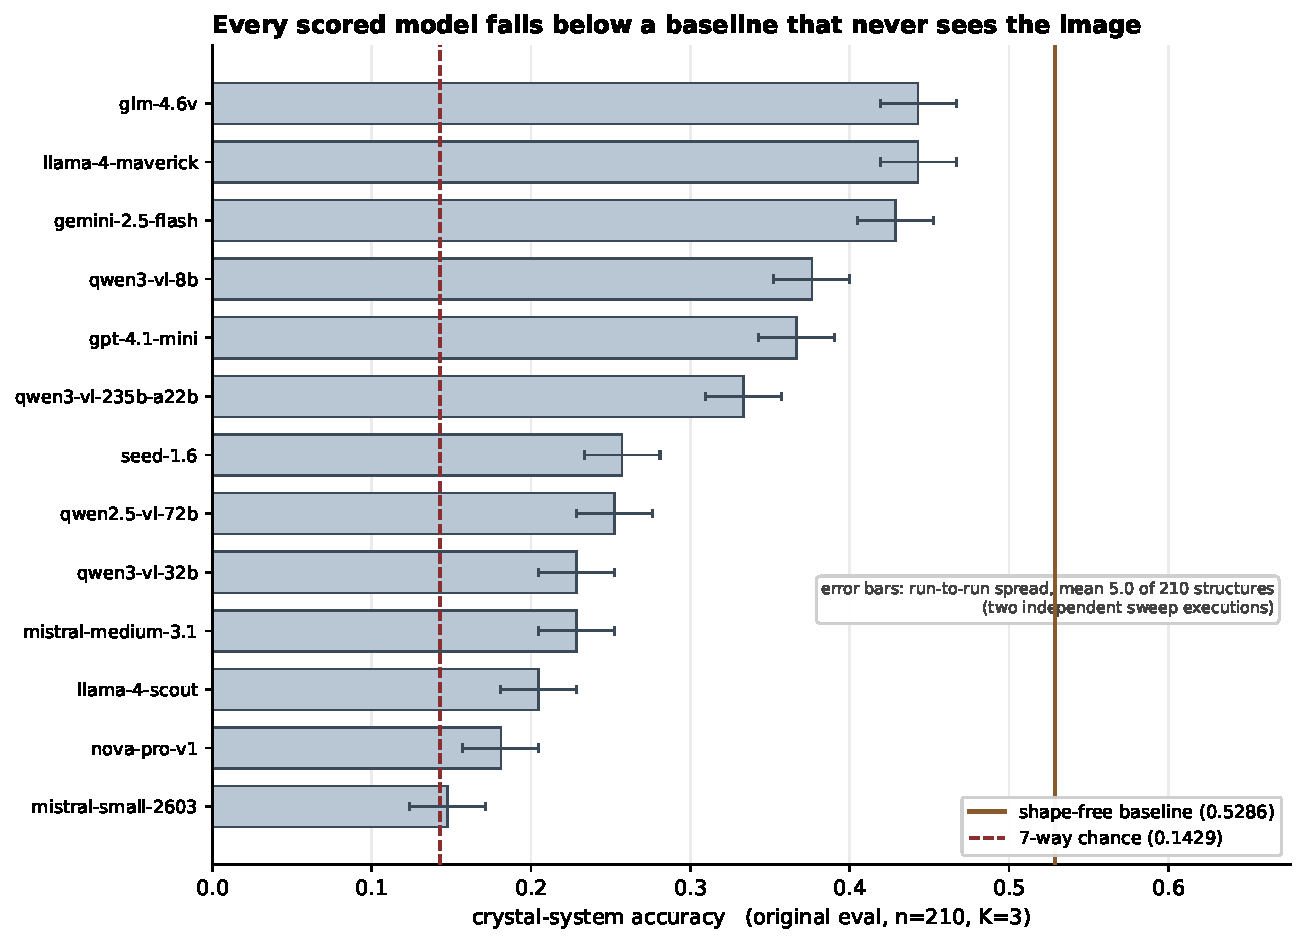
\includegraphics[width=0.8\linewidth]{figures/leaderboard.pdf}
\caption{Zero-shot leaderboard, original sample, $n=210$, $K=3$, 13 scored models across eight vendors.
Dashed line: the shape-free baseline (atom count, density, cell volume) on this sample. Error bars: the
measured run-to-run spread of $K{=}3$ majority voting.}
\label{fig:leaderboard}
\end{figure}

\textbf{A modality-matched reference.} A cell-metric random forest reaches 0.8952 on crystal system, above
every model. This reproduces an established capability rather than contributing one; it is not comparable
to \citet{cryspnet2003}, which predicts symmetry from composition alone, the opposite input and a harder
problem.

\paragraph{The strongest model arm, and what is not claimed for it.}
The 0.6905 figure is a supervised-then-GRPO arm on \texttt{Qwen/Qwen3-VL-8B-Instruct}, reported as a
single-seed point estimate at $K{=}8$; the same adapter gives $139/210 = 0.6619$ at $K{=}3$. It sits inside
the reference arm's across-seed spread ($0.590 / 0.567 / 0.686$), exceeding that arm's best seed by one
structure at $K{=}8$ and trailing it by five at $K{=}3$, so \emph{we make no claim that this arm improves
on the reference arm}. It is used only as the model side of the ceiling-to-model gap (200 against 145,
discordance $61{:}6$, $p = 1.5\times10^{-12}$), which survives any seed in the observed spread. The
three-seed extension was cut; its record and the quantitative argument for the cut are in the
supplementary.

\subsection{Perception versus symbolic residual}
\label{sec:residual}

\textbf{Exact geometry does not close the gap.} Supplying ground-truth geometry as text (the CIF-supplied
condition of \citet{xcrys2506}, cited as prior use) lifts every model substantially, and none reaches the
oracle: the best is 0.8524 against 0.9524 (Figure~\ref{fig:ladder}, left). The pre-registered decomposition of Definition~\ref{def:ladder}
gives a median perception share of 30.9\% across the 14 models scored under the coordinate condition, with
the symbolic residual the larger of the two for 12 of them (Figure~\ref{fig:ladder}, right); the two columns of Table~\ref{tab:rungs} differ
in perception share by a factor of six. Only the two strongest models are perception-dominated, and the
share tracks pixel accuracy (Spearman $\rho = -0.6439$, $p = 0.0130$). \emph{The bottleneck moves with
model strength}: a more precise statement than either single attribution, and one visible only because the
oracle fixes the top of the ladder.

\begin{figure}[t]
\centering
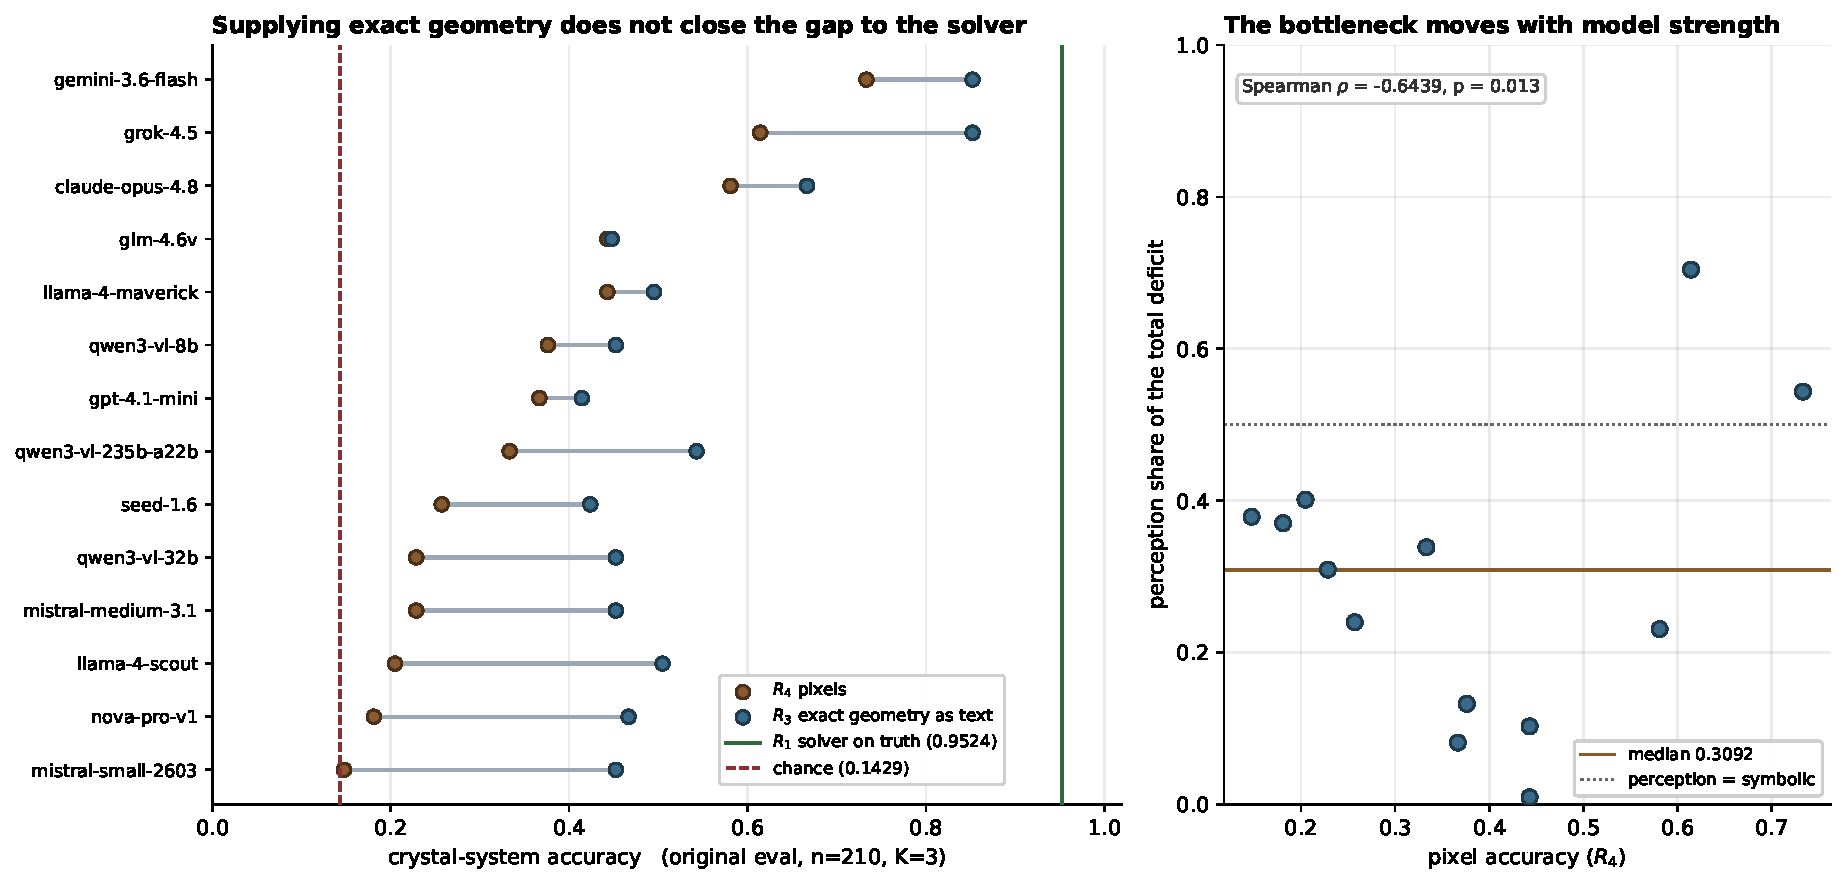
\includegraphics[width=0.8\linewidth]{figures/ladder.pdf}
\caption{Left: per-model $R_4$ (pixels) and $R_3$ (exact geometry as text) on the original evaluation
sample ($n=210$, $K=3$), rungs as in Definition~\ref{def:ladder}, with the $R_1$ oracle and seven-way
chance drawn; $R_2$ is omitted (unscored under its pre-registered gate). Right: perception share of the
total deficit against pixel accuracy, with the median and the perception-equals-symbolic line drawn.}
\label{fig:ladder}
\end{figure}

\textbf{A control pair makes $R_3$ readable.} Removing the images and leaving only the chemical formula
collapses every scored model toward seven-way chance (mean 0.1487 over the 13 models scored under the
image-removal control). Removing the images and supplying full geometry lifts every scored model to
between 0.4143 and 0.8524.
The two conditions differ in one thing, so the lift is the geometry rather than text-mode prompting; the
geometry prompts are also shorter than the five-image prompts they beat, which rules out a length artefact.

\subsection{Controls and intermediate verification}
\label{sec:controls}

\textbf{The symbolic residual is an upper bound, and we tested it.} A residual against a solver may include
long-list handling rather than symmetry reasoning. Regressing per-structure $R_3$ correctness on
conventional-cell atom count over the same records (no new model calls): pooled over the 14 scored models
and 2940 model-structure pairs, Spearman $\rho = -0.0908$ at $p = 8.1\times10^{-7}$; 13 of 14 models are
negative, and accuracy falls from 0.5551 on cells at or below the median 14 atoms to 0.5129 above it
(Fisher $p = 0.0241$). The pre-registered confound control does not rescue it: atom count correlates with
crystal system ($\rho = -0.1866$), but the mean within-system association is $-0.1053$, stronger than the
pooled figure rather than attenuated, so the effect is not symmetry difficulty in disguise. We therefore
report the symbolic residual as an upper bound on a symmetry-reasoning deficit, not as a measurement of
one. Nothing here touches the oracle-to-model gap, which is measured against pixels.

\textbf{A learned extractor fabricates its output.} Substituting a strong model as the extraction stage,
prompted for species and positions with the symmetry question withheld, and having a weaker model answer
from that text yields 0.1429. That arm predicted two of seven classes and its accuracy equals the majority
stratum's base rate, so it measures nothing. The informative measurement is the intermediate, scored
directly against ground truth: median recall 0.0000, with 105 of 206 structures having not one emitted atom
within tolerance of a real one, despite a median of 48 well-formed atoms per structure. A colour-threshold
blob detector achieves median recall 0.400 on the same task. Downstream accuracy alone would have read this
as bad reasoning. \emph{A two-stage pipeline whose intermediate cannot be checked will attribute
fabrication to reasoning}, which is the argument for the instrument.

\textbf{The models do use the image.} A benchmark on which models score poorly invites the objection that
they are pattern-matching the prompt rather than reading the figure. We ran the image-absent control that
\citet{cotdeg2604} made standard: the identical prompt carrying the chemical formula and no renders. Every
scored model collapses toward seven-way chance (mean 0.1487), and the paired per-structure difference is
significant for 10 of the 13 models scored under the image-removal control (Figure~\ref{fig:noimage}); the
strongest model loses 0.5714. The three nulls are the three weakest models, two of which are not above
chance even with images, so those are floor effects rather than evidence of formula lookup.

\begin{figure}[t]
\centering
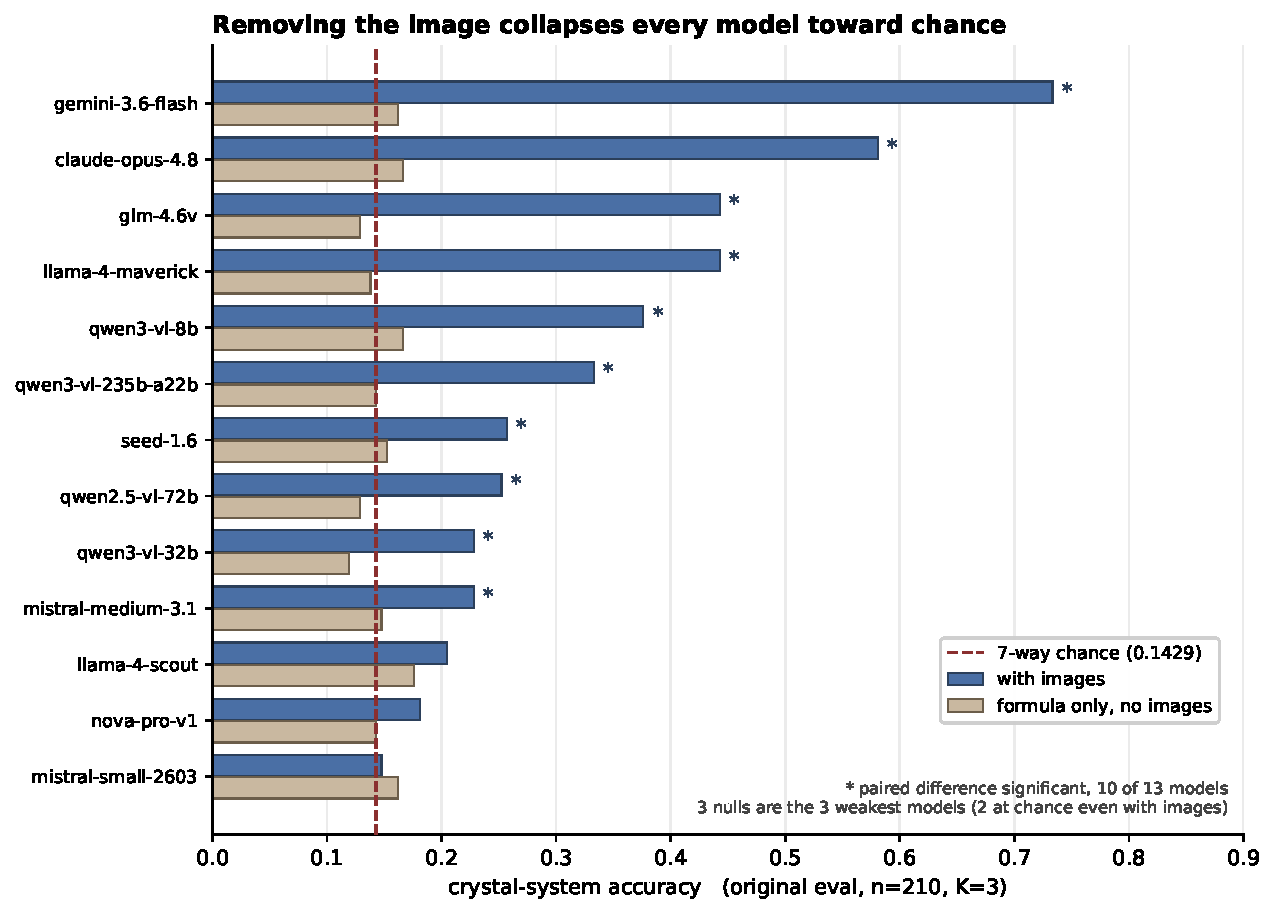
\includegraphics[width=0.8\linewidth]{figures/noimage.pdf}
\caption{Image-removal control: each model answered the identical prompt with the five renders and with the
chemical formula alone, paired per structure (original sample, $n=210$, $K=3$, 13 scored of 16 attempted).
Stars mark models whose paired difference is significant; the dashed line is seven-way chance.}
\label{fig:noimage}
\end{figure}

\textbf{A baseline comparison we previously reported does not survive scale-up, and we retire it.} On the
original sample every model falls below a shape-free baseline reading only atom count, density and cell
volume (0.4429 against 0.5286, one-sided $p = 0.0078$). We regenerated the evaluation set at $n = 1933$
under identical rules: same composition exclusion, verified zero overlap with training and both earlier
samples, stratified 285 per system before quarantine, with 62 structures (3.11\%) removed for label
instability under the tolerance sweep. On that sample the baseline falls to 0.2054. Because the new draw
also has larger cells (median 38 atoms against 14), we ran a size-matched control restricted to the
original's 95th percentile: the baseline is 0.2205 there, so the shift is not a cell-size artefact.
\emph{The 0.5286 was a property of the original draw, not of the task}, and the below-baseline claim is
scoped to that sample rather than asserted generally.

The same control shows the oracle's apparent drop at scale \emph{is} a cell-size effect: 0.8774 on the full
sample but 0.9459 at matched cell size, within 0.0065 of the original. More atoms per cell means more
projective coincidence and more correspondence ambiguity, which is the failure set of
Proposition~\ref{prop:ident}. The ceiling-to-model gap, which is what this paper rests on, therefore
survives scale-up (0.9459 against 0.4429), while the baseline comparison does not.

\textbf{Run-to-run spread is a benchmark property.} An unplanned second execution of the sweep gives a mean
absolute difference of 5.0 structures and a maximum of 11, so adjacent leaderboard rows are not separable
and the ordering is not exact.

Two axes are reported in full in the supplementary and summarised here, because both end by disclaiming
themselves and neither carries a main-text claim.

\textbf{Cue sufficiency.} Whether the conventional-cell metric alone determines the crystal system splits
the samples $140/70$ and $141/69$ and is a stable property of the render convention with no accuracy
mechanism attached: an earlier claim that pixel accuracy simply drops on the ambiguous stratum failed four
independent tests and is withdrawn. A contrast against a cell-metric control does widen on that stratum for
all three frontier models on both samples (Figure~\ref{fig:cuesuff}), but the stratum is $60/70$ and
$58/69$ hexagonal-or-trigonal, so the finding is close to a restatement of that one degeneracy, and the
degeneracy-removed residual rests on $n=10$ and $n=12$.

\textbf{One generation of model progress.} It does not erase the axis (Figure~\ref{fig:generational}): from
gemini-2.5-flash to gemini-3.6-flash the newer model gains more on the ambiguous stratum in raw terms but
closes less of its headroom to the oracle (54.1\% against 64.0\%), and one model pair is a comparison
rather than a trend.

\subsection{Render conventions}
\label{sec:conventions}

Two of the frozen protocol's geometric choices are information-suboptimal, measured by the oracle.
Perturbing the cameras off the principal axes raises the ceiling from 0.9524 to 0.9952 ($p = 0.0039$,
monotone: nine structures gained, none lost). Supplying the oracle the shipped protocol's $2\times2\times2$ tiling instead of the single conventional cell
\emph{costs} it twenty-two structures, 0.9524 against 0.8476 ($p < 10^{-6}$, gained 0, lost 22), because
tiled copies project onto coincident pixels and a triangulating reader cannot separate them; both effects are instances
of the coincidence failure set of Proposition~\ref{prop:ident}.

Neither correction reaches the models. Four strong models across five conventions on a stratified
70-structure subsample give zero significant changes in 16 paired comparisons, with near-symmetric
discordance in every convention and inconsistent direction within conventions. Power is low and we state it
per comparison rather than as a single number. The test is a paired exact binomial on discordant pairs;
discordance averages 6.3 of 70, and significance is reachable in only 9 of the 16 comparisons, the other 7
having too few discordant pairs for any split to reach $p<0.05$ (Appendix~\ref{app:stats} gives the
procedure and the per-comparison minimum detectable differences, which run 0.0857 to 0.1286 across the 9
comparisons where significance is reachable at all, against a largest observed effect of 0.0857). \emph{We therefore do not claim the null bounds the effect at any
particular size.} What it supports is that no convention produced a detectable change, and that for seven
comparisons the design could not have detected one. An intervention that adds information a model cannot
use is evidence about the model.

\textbf{What the protocol withholds is small and redundant.} The oracle of Section~\ref{sec:oracle} assumes
ideal extraction, so a separate measurement is needed to say what the images themselves hide. Classifying
every occluder by whether it hides a symmetry-equivalent copy shows most occlusion hides nothing
recoverable, and because triangulation needs only two clear views, under 1\% of atoms are untriangulable
from the frozen view set (0.26\% and 0.87\%).
Removing informative occlusion from the oracle's input changes no classification at all
(Figure~\ref{fig:conditions}), while the pre-registered redundant-only control changes several, so render
adequacy is established and the deficit is forced onto the model.
